\documentclass[tikz]{standalone}
\usepackage{tikz}
\usepackage{fourier}
\usepackage{physics}
\usetikzlibrary{shapes.geometric}
\usetikzlibrary{calc}

\begin{document}
\begin{tikzpicture}
    % Spherical harmonic plots
    \node[inner sep=0] at (0, 0) {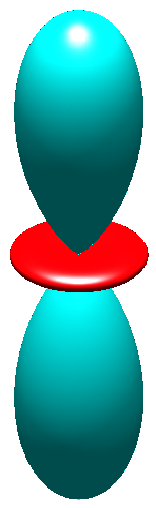
\includegraphics{../gfx/UN-spherical.pdf}};
    \node[inner sep=0] at (7, 0) {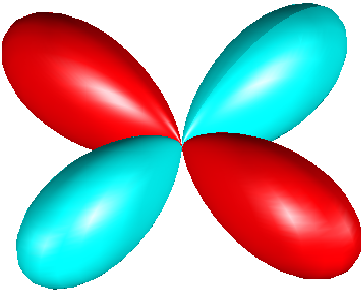
\includegraphics{../gfx/BN-spherical.pdf}};
    \node[inner sep=0] at (16, 0) {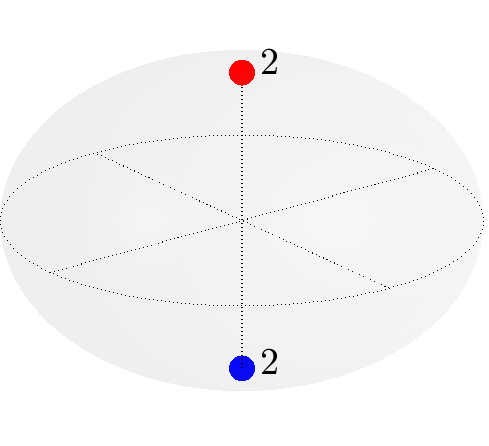
\includegraphics{../gfx/UN-Majorana.pdf}};
    \node[inner sep=0] at (25, 0) {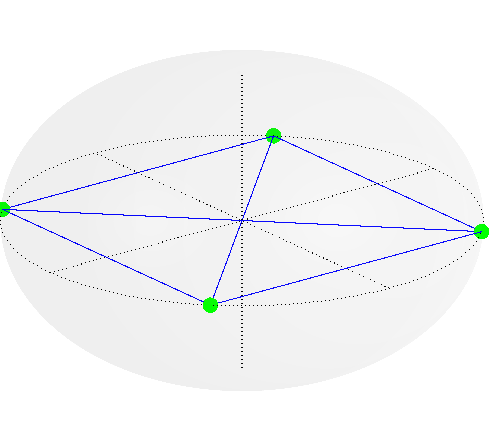
\includegraphics{../gfx/BN-Majorana.pdf}};

    % Colour bar
    \node[rotate=90] at (-3.5, 0) {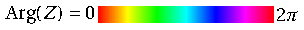
\includegraphics[scale=1.8]{../gfx/compiled_hsv.pdf}};
    \node at (30, 0) {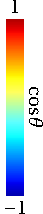
\includegraphics[scale=1.8]{../gfx/compiled_jet_majorana.pdf}};

    % Labels
    \node at (0, -5) {\Huge (a)};
    \node at (7, -5) {\Huge (b)};
    \node at (16, -5) {\Huge (c)};
    \node at (25, -5) {\Huge (d)};

    % UN labels
    \draw[-, line width=2] (0, 4.1) -- (0, 5.1) node[above] {\Huge \(\hat{\vb{d}}\)};
    \draw[->, line width=2] (1.15, -0.05) -- (1.8, -0.05) node[right] {\Huge \(C_2\)};

    % BN Labels
    \draw[->, line width=2] (7, 0) -- (7, 2) node[above] {\Huge \(C_4\)};
    \draw[->, line width=2] (9.6, 2.2) -- (10.2, 2.8) node[above] {\Huge \(C_2\)};
    \draw[->, line width=2] (8.4, 0.1) -- (10, 0.1) node[right] {\Huge \(C_2'\)};

    % Orientation
    \draw[->, line width=2] (-2.8, -4) -- (-2.8, -3) node[above] {\Huge \(z\)};
    \draw[->, line width=2] (-2.8, -4) -- (-1.8, -4) node[right] {\Huge \(x\)};
    \draw[->, line width=2] (-2.8, -4) -- (-2.2, -3.5) node[right] {\Huge \(y\)};

    % Spinor labels
    \node at (16, 3.7) {\Huge \(\zeta^\text{UN} = (0, 0, 1, 0, 0)^T\)};
    \node at (25, 3.7) {\Huge \(\zeta^\text{BN} = (1, 0, 0, 0, 1)^T/\sqrt{2}\)};

\end{tikzpicture}
\end{document}

